\documentclass{article}
\usepackage{graphicx} % new way of doing eps files
\usepackage{listings} % nice code layout
\usepackage[usenames]{color} % color
\usepackage{float}
\definecolor{listinggray}{gray}{0.9}
\definecolor{graphgray}{gray}{0.7}
\definecolor{ans}{rgb}{1,0,0}
\definecolor{blue}{rgb}{0,0,1}
% \Verilog{title}{label}{file}
\newcommand{\Verilog}[3]{
  \lstset{language=Verilog}
  \lstset{backgroundcolor=\color{listinggray},rulecolor=\color{blue}}
  \lstset{linewidth=\textwidth}
  \lstset{commentstyle=\textit, stringstyle=\upshape,showspaces=false}
  \lstset{frame=tb}
  \lstinputlisting[caption={#1},label={#2}]{#3}
}


\author{Jiasen Zhou, Jon Johnston}
\title{Lab 9: Integrating Fetch and Decode}

\begin{document}
\maketitle

\section{Executive Summary}
The purpose of this lab is to design and simulate the datapath with the iExecute module integrated into it. Datapath.v now contains the 

\section{Test Report}
To verify operation of these module, this lab requires one test bench. 
\begin{enumerate}
	\item datapath
\end{enumerate}



\pagebreak

\begin{figure}[H]
	\begin{center}
		\caption{Expected Results of the datapath test.}\label{fig:ert_datapathtest}
		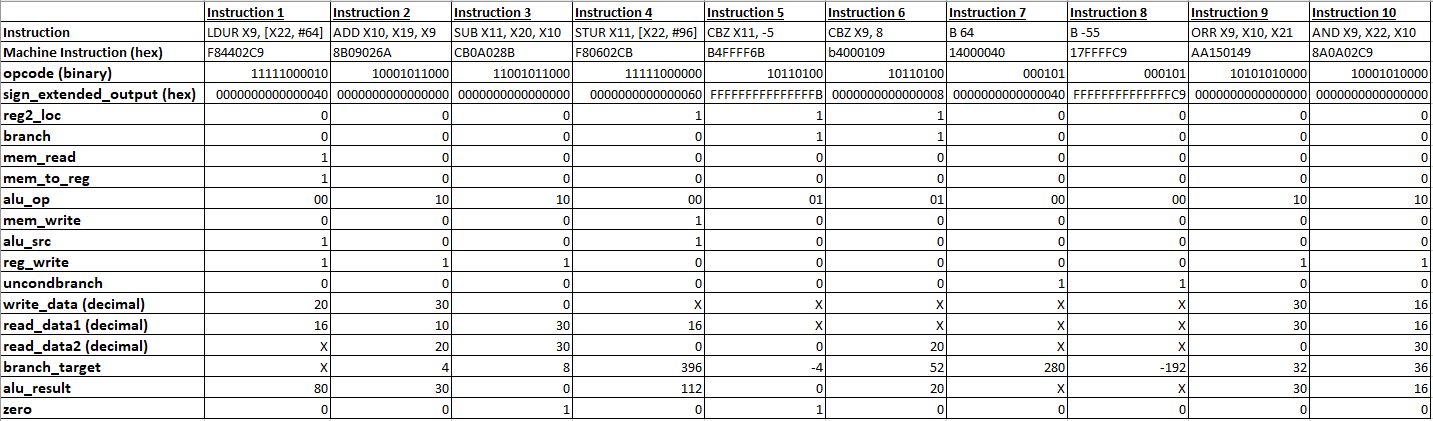
\includegraphics[width=1.0\textwidth]{../images/DatapathExpected9.png}
	\end{center}
\end{figure}

\begin{figure}[H]
	\begin{center}
		\caption{Timing diagram for the datapath test.}\label{fig:datapathtest}
		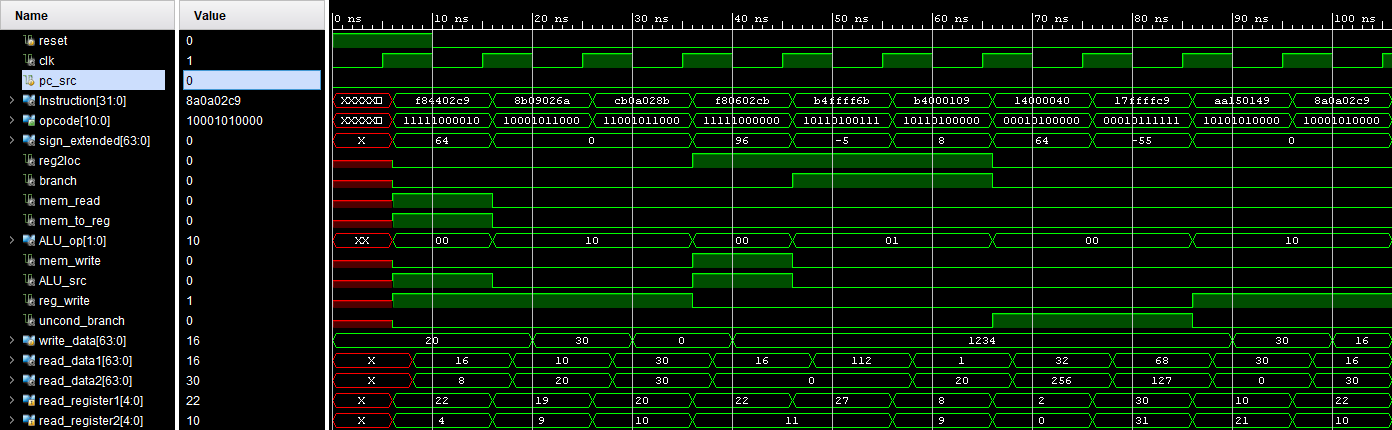
\includegraphics[width=1.0\textwidth]{../images/DatapathSimulation.png}
	\end{center}
\end{figure}


\section{Code Appendix}
\Verilog{Verilog code for testing the datapath.}{code:regtest}{../code/2_decode/datapath.v}
\end{document} 